\chapter{Implementation}

\section{Issues Encountered During Implementation}

\subsection{Creating Tables Using Bootstrap}

Initially it was decided to create the SQL tables during visualisation using the Bootstrap 5 grid system. Using a series of rows and column in a flexbox it can layout and align the content responsively. This seemed like a good tool for creating tables because it allowed the creation of custom layouts for tables and it would give more freedom for styling and highlighting since, it is not as restrictive as a HTML table element. 

Also HTML tables were not initially used because the idea was to create tables that did not have any contents inside of them apart from headers, so the table cells would be empty which would not be desirable. The application would not be able to parse "INSERT" statements which means no entries will be added to the tables so it would lead to empty rows in the table.

Later on in the implementation of this tables, when the parsing was sophisticated enough to parse large tables, the problem emerged of Bootstrap shifting the layout of the tables and compressing it's columns together to look like rows on smaller screen or if the window was resized. 

The grid system is useful when building layouts for mobile-first designs, the layout of the webpage changes when the size of the screen is changed. However, for this project, learners are not going to be writing their SQL databases on a mobile device, or devices with very small screen so it is not very useful and the structure of the tables should not change when the window size is altered. 

\begin{figure}[h!]
	\centering
	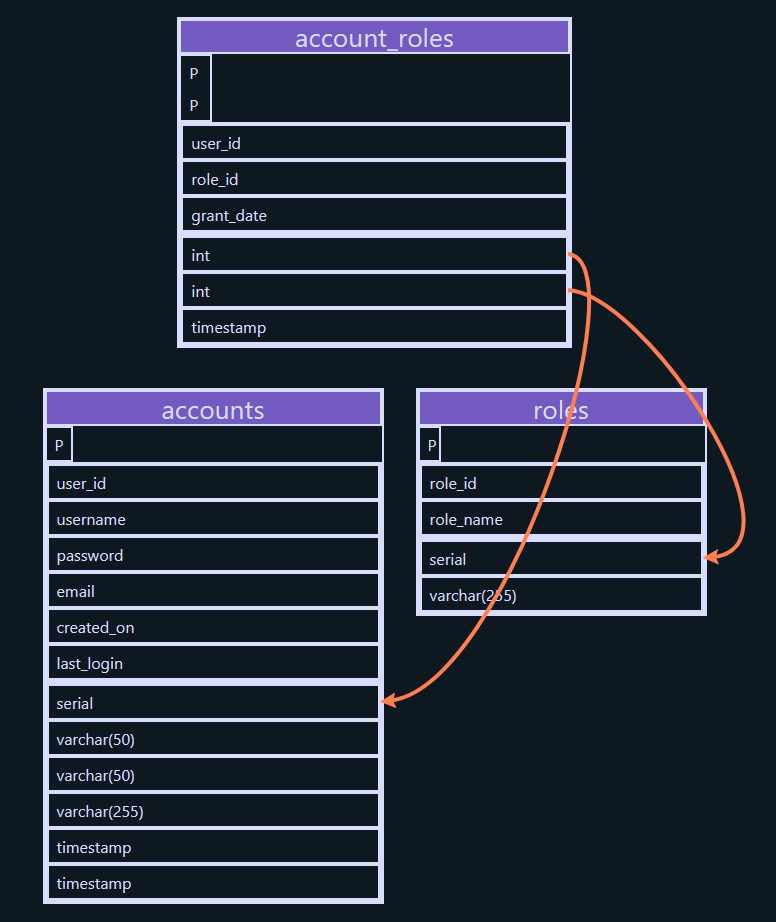
\includegraphics[scale=0.5]{postSquash}
	\caption{Visualisation of tables showing the column being compressed to look like rows in a single column due to the flexbox responsive resizing.}
	\label{fig:squash}
\end{figure}

This problem was solved by going back to using HTML table elements and dynamically creating tables from the table objects. This solution was slightly harder to implement however, the and layout was much better since Bootstrap did not resize the table element. 

This was because the entire table is viewed as an element which prevents it from being changed when the window is resized, compared to the previous implementation, which had a table comprised of multiple column and row elements which were resized and the flexbox layout was altered. Bootstrap provides styling classes for these new tables which made the styling easy to make look like the previous table design.

\begin{figure}[h!]
	\centering
	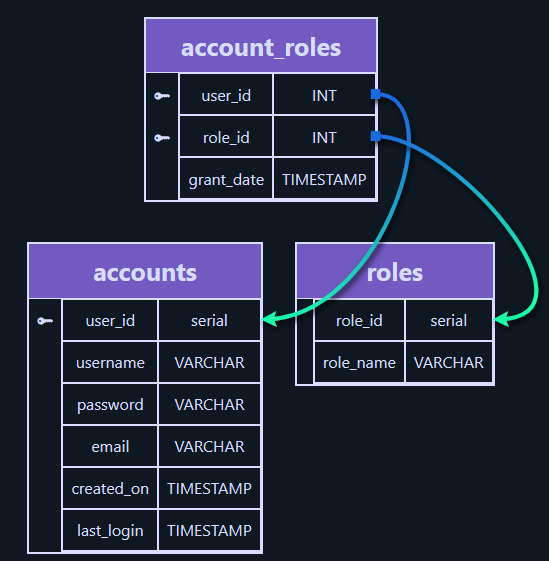
\includegraphics[scale=0.7]{newPostSquash}
	\caption{Visualisation of tables after using HTML table elements, there is not resizing or changing of layout after the window is resized.}
	\label{fig:afterSquash}
\end{figure}

\subsection{Early Stages of Parsing}

The early stages of parsing used simple checking of strings and struggled separating spaces and punctuation properly, it used regular expressions that were hard to read and were prone to break when more syntax checking was added. Using the tokenising library made it easier to write parsing logic since tokens made it much easier to sanitise the text and separate each word.

Parsing was a lot more complex than initially thought, there were lots of edge cases for SQL statements and an immense complexity in the number of possible statements, and combination of flags in those statements. This meant that a lot of time and effort went into writing parsing logic for only a few SQL statements, this was challenging however was completed with enough time. 

\subsection{Drawing arrows library}

Drawing lines between two HTML elements was something that had to be done to represent foreign key relationships between tables. One possible way to do was to use a HTML canvas and draw lines using the position of elements on the webpage. However, this was difficult to style correctly in order to match the design of the website and would require more work to create a function to do so. Instead, a library called LeaderLine \cite{leaderLine} was used to draw an arrow between two elements. The styling of this arrows was much easier to do and it also included some implementation for animations which made the design look much better than the HTML canvas lines.

\subsection{Drawing Tables on the webpage}

Drawing the tables in a way that was easy to understand was difficult because the order or layout the tables are displayed in, plays a key role in how easy a database can be understood. It was first implemented to display the tables in the order in which the tables appeared in the SQL text file since it seemed like a most logical solution. 

This was done because the learners will expect the tables to be displayed in this order however, once foreign key arrows were implemented, the tables had arrows stretch across them because the tables were horizontally laid out. 

It also meant that arrows had to be very long, spanning across the webpage since tables that were joined together were not were not always defined together in the SQL file or text. This was quite confusing to try to understand and a decision was made to display them in a more organised structure. 

\begin{figure}[h!]
	\centering
	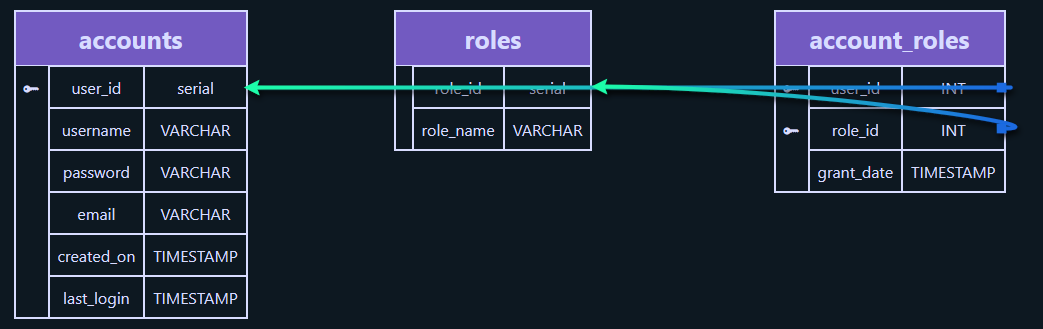
\includegraphics[width=\textwidth]{overlap}
	\caption{Visualisation of tables depicting overlap between the tables and foreign key arrows preventing text in columns to be readable.}
	\label{fig:overlap}
\end{figure}

\subsection{Representation of Missing Primary Keys}

The first implementation of feedback to the user for flaws was red highlighting tables that had no primary key. The key column of the table that had no primary key constraint was highlighted red to show that there was a flaw present in the table design.

A missing primary key is a integral part of the design that should be fixed with a high priority and this should be conveyed to the user. However, the first implementation of this did not make it clear what was missing which might be confusing to the user.

\begin{figure}[h!]
	\centering
	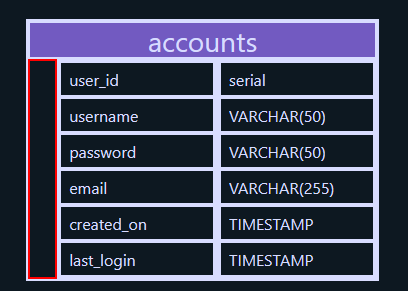
\includegraphics[scale = 0.8]{missingFK}
	\caption{Visualisation of a table with no primary key constraint showing the key column border being highlighted red.}
	\label{fig:missingFK}
\end{figure}

This needed to be visually more informative and have some kind of prompt to the user to explain what the flaw with the table is. A later implementation addressed these issues by instead of just highlighting the key column, it changed the colour of the entire table border to be red and when the user hovers over the table there will be a tooltip that shows, informing the user that there is a missing primary key constraint in this table. This is a much better implementation since it gives instant feedback to the user about the flaw in the design as soon as it is visualised. 

\begin{figure}[h!]
	\centering
	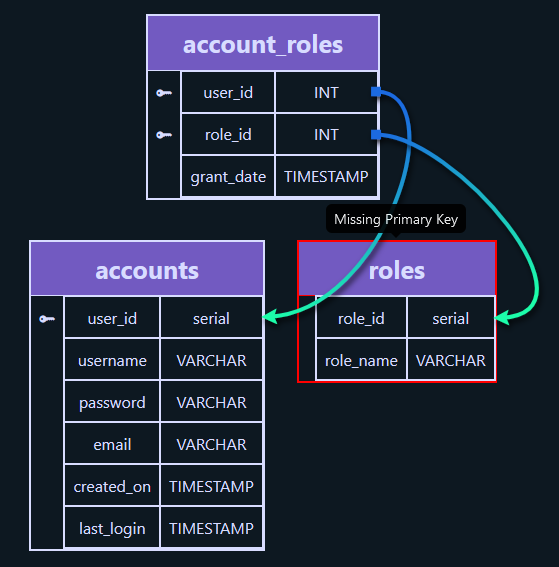
\includegraphics[scale = 0.8]{missingFKNew}
	\caption{New implementation of informing the user that a table has no primary key constraint using a Bootstrap tooltip.}
	\label{fig:missingFKNew}
\end{figure}

\subsection{Implementing Highlighting of Text in a HTML TextArea}

A HTML text area used in the website input form to enter the SQL text by the user. In order for this text area to be user-friendly, there should be some sort of feedback to the user if the SQL code they entered has some SQL syntax errors. And if there are any syntax errors it should inform the user as to where the syntax errors are in the code they entered. This is important because an SQL learner will not be able to easily spot where the errors are in the SQL code, since they are not familiar with the SQL syntax. 

\begin{figure}[h!]
	\centering
	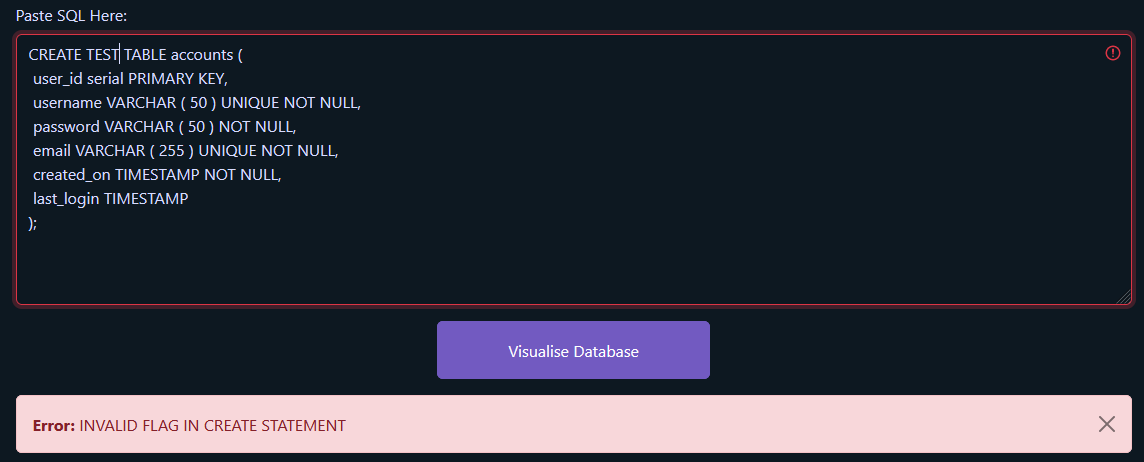
\includegraphics[width=\textwidth]{textArea}
	\caption{Initial implementation of the text area, including validation and syntax error alerts.}
	\label{fig:textArea}
\end{figure}

The HTML text area does not natively have the functionality to highlight text that is entered inside of it, any markup to the text would appear as plain text. A possible solution to this problem is to implement a rich text editor in the webpage and replace the text area with it, rich text areas can provide implementation to highlight and mark up text. However building a rich text editor from scratch is difficult to do since even basic functionality is demanding to implement \cite{highlightText}.

Another solution to this problem would be embedding an already functioning rich text editor in the webpage. This approach would require styling it and cutting down all of the features down only to the simply highlighting, from this evaluation it was decided to create a simple work around for the lack of functionality of the HTML text area. 

This was done by creating a "fake" text area under the current one that only looked like a text area although it was a div element, and since it was overlaid over the text area, it was not perceivable by the user. The goal of this text area is to highlight the text and match the position of it to the text area on top of it to make it seem like one component on the webpage. 

This div was styled so that it was identical to the text area and it's background was set to transparent so it did not interfere with the overall design. The highlighting was done by creating span elements of the words that had to be highlighted, these span elements had styling to change the colour of it's background. So from the point of view from the user, they can see the text from the text area and the highlighting done by the background of the span elements.

This proved to be quite easy to implement and provides the solution to the problem without having to write a rich text editor or implement one. This solution to the problem was inspired by an article \cite{fakeTextArea}.

\begin{figure}[h!]
	\centering
	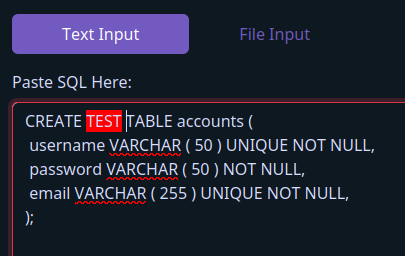
\includegraphics[scale = 1]{highlightedTextArea}
	\caption{Later implementation of highlighting the origin of the syntax error in the input text area.}
	\label{fig:highlightedTextArea}
\end{figure}

\newpage

\section{Review of Requirements}

The initial requirements are all mostly met apart from the functionality that is outside the \textit{\hyperref[subsec:scope]{scope}} of this project that is mentioned previously in the report. 

\begin{center}
	\captionof{table}{\label{fig:reviewOfImplementation}Table reviewing the initial table of requirements.}
	\setlength\extrarowheight{2pt}
	\begin{tabularx}{\textwidth}{|X|X|X|}
		\hline
		\textbf{Functional Requirement Number} & \textbf{Functional Requirement Name} & \textbf{Review of Requirement} \\
		\hline
		FR-1 &  Enter SQL into website form. & The user can enter their SQL in either text or file form. This can be done by either entering text into the text area or uploading a file into the file picker. The website accurately processes the data that the user provides and there are restrictions to the file types that the user can upload. \\
		\hline
		FR-2 & Validate entered SQL. & Once the data has been entered the SQL is validated and feedback is given to the user. If there are syntax errors in the SQL, alerts are created to inform the user as well as red highlighting of the text area.\\
		\hline
		FR-3 & Visualise entered database. & The entered database is visualised by creating tables and the links between them. They are laid out in a way to make it easy to understand the structure of the database.\\
		\hline
		FR-4 & View highlighted syntax after visualising. & Once the database has been visualised, the "Syntax View" tab can be selected to find the highlighted and indented SQL that had been entered before. \\
		\hline
		FR-5 & The user can filter through data types of columns in the "Syntax View". & In the "Syntax View" tab there are filters that can be checked to highlight the data types, all of these data types in the syntax highlighter are highlighted to a green colour to separate them from the rest to make it easier to distinguish them from the rest. \\
		\hline
		FR-6 & The user can view the flaws of the database. & Once the database has been visualised, the "Problem View" tab can be selected with a list of flaws that the database might have, if there are no flaws detected then the user is prompted with a message. \\
		\hline
		FR-7 & The user can view the advice on how to fix the flaws identified. & In the "Problem View" tab the user can expand each flaw and find information on how to fix the flaw that was identified in the database. \\
		\hline
	\end{tabularx}
\end{center}